\subsection*{Задание 1.1}

\underline{Условие:} Все потоки случайных событий считать пуассоновскими. Если все операторы заняты, звонок теряется. Рассчитать минимальное число операторов, при котором доля отказов не превышает 25\%, 10\%, 5\%, 1\%.
Построить график вероятности отказа от числа операторов. Построить график, иллюстрирующий коэффициент загрузки операторов в зависимости от их числа.
\\

\underline{Решение:}

Вероятность того, что ни один из операторов не будет занят, рассчитывается по формуле 1:

\begin{equation}
    P_0 = \frac{1}{\sum_{i=0}^N \frac{\lambda^i}{i! \mu^i}}
\end{equation}

, где

$P_0$ - вероятность того, что ни один из операторов не будет занят, 

$N$ - количесво операторов,

$\lambda$ - интенсивность поступления заявок, 

$\mu$ - интенсивность обработки заявок.
\\

Для расчета вероятности отказа воспользуемся формулой:

\begin{equation}
    P_{den} = \frac{\lambda^i}{i! \mu^i}P_0
\end{equation}

, где $P_den$ - вероятность отказа системы.
\\


Для расчета среднего количества занятых операторов используем формулу: 
\begin{equation}
    \overline{N} = \sum_{i=0}^N i P_i
\end{equation},
где \\ $\overline{N}$ - среднее количесво занятых операторов в системе\\
$P_i$ - вероятность отказа $i$-го оператора. 

Коэффицент загрузки операторов считается по форумуле 
$k = \frac{\overline{N}}{N}$, где $N$ - текущее число операторов.

\begin{figure}[h!]
    \centering
    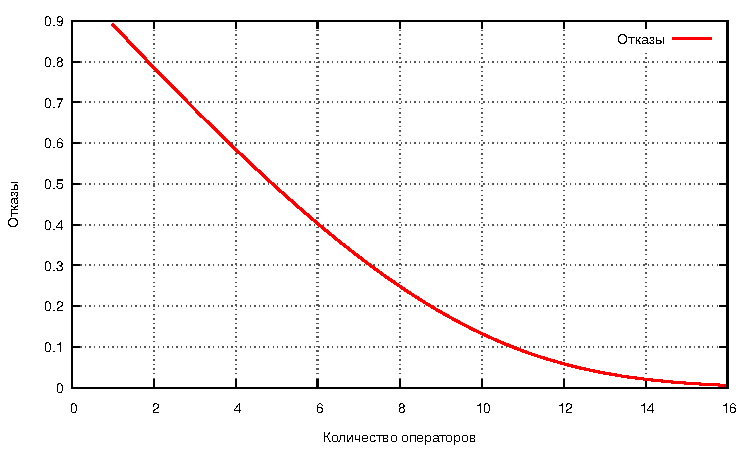
\includegraphics[width=0.7\textwidth]{z1.1/refuses.pdf}
    \caption{Зависимость отказов системы от количества операторов.}
\end{figure}

\begin{figure}[h!]
    \centering
    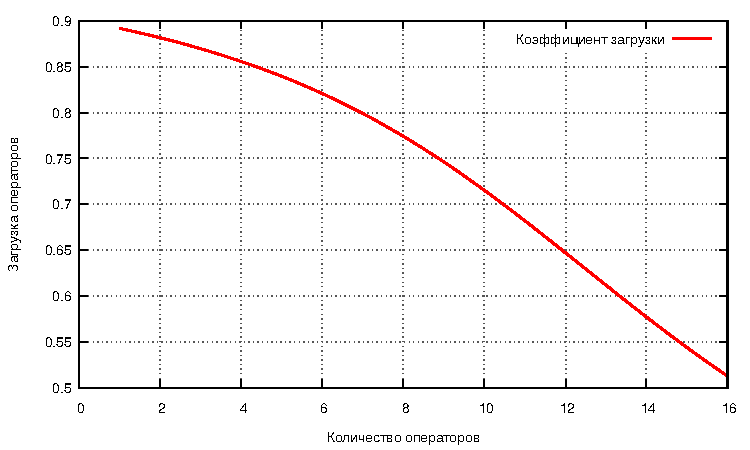
\includegraphics[width=0.7\textwidth]{z1.1/koeffzagrop.pdf}
    \caption{Зависимость отказов системы от количества операторов.}
\end{figure}